\documentclass[a4paper,twoside,12pt]{extarticle}

%Characters and language
\usepackage[Latin1]{inputenc}
\usepackage[T1]{fontenc}
\usepackage[english]{babel}

%Page setup
\usepackage[top=6em,bottom=6em,left=3em,right=3em]{geometry}
\usepackage[pdftex,
  bookmarks=true,
  bookmarksnumbered=true,
  pdfstartview=FitH,
  pdfpagelayout=SinglePage,
  colorlinks=true,
  linkcolor=blue,
  urlcolor=blue,
  pdfborder={0 0 0}
]{hyperref}

%Misc
\usepackage{graphicx,beton}
\graphicspath{{Graphics/}}
\def\bfdefault{m}

\title{\bfseries Organ Builder\\User manual}
\date{\today}
\author{\href{mailto:vincent.forman@gmail.com}{Vincent Forman}}

\begin{document}

\vfill
\maketitle
\vfill
\begin{center}
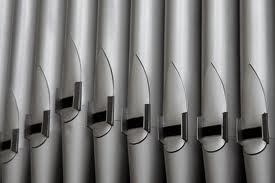
\includegraphics[width=0.6\textwidth]{Pipes.png}
\end{center}
\vfill
\tableofcontents
\vfill
\newpage

\section{Introduction}

Copyright \copyright{} 2014 Vincent Forman (original author)

\subsection{License}

This program is free software; you can redistribute it and/or modify it under the terms of the GNU General Public License as published by the Free Software Foundation; either version 3 of the License, or (at your option) any later version. 

This program is distributed in the hope that it will be useful, but WITHOUT ANY WARRANTY; without even the implied warranty of MERCHANTABILITY or FITNESS FOR A PARTICULAR PURPOSE. See the GNU General Public License for more details. 

You should have received a copy of the GNU General Public License along with this program; if not, write to the Free Software Foundation, Inc., 51 Franklin Street, Fifth Floor, Boston, MA 02110-1301 USA.

\subsection{Purpose}

The Organ Builder program allows the user to generate \textit{organ definition files}, to be used with the GrandOrgue software. If you have an organ sampleset which is only compatible with proprietary software, this program can greatly speed up the process of making it compatible with GrandOrgue.

\subsection{File types}

The Organ Builder program features its own file format: organ definition projects (\verb|.odp| files). The program can export a project in GrandOrgue format (\verb|.organ| files) at any time through the main menu.

\section{User interface}

The user interface features three main tabs and a main menu bar. File operations are available through these menus.

Most design operations will consist in drag and drop operations with the mouse.

In what follows, the term \textit{button} will refer to either a \textit{drawstop} or a \textit{piston}, depending if it is dropped on a drawstop panel or a piston panel. The difference is purely cosmetic.

\subsection{Configuration}

On the first run, the user will be given the ability to choose a preferred language. For now, only two translations are available for Organ Builder:
\begin{itemize}
\item English;
\item French.
\end{itemize}
If you would like to contribute and write new translations, you can contact the author for details.

The user can also choose if paths to files (wave samples and such) are to be stored as absolute paths in \verb|.odp| files, or relative to the project folder. This setting is useful for project files which are to be distributed, and wont affect the generated \verb|.organ| files.

\subsection{The \textit{Organ structure} tab}

This tab will let the user define the general structure of the organ: number of keyboards and keys, pedals, couplers, etc. Some visual settings are also available here, applying to certain types of organ objects (eg. enclosure pedals, couplers, etc.).

The philosophy of the program is that, like in most real-world organs, each manual is associated to its own division, featuring a number of attributes: existence of a tremulant, existence of an enclosure, etc. This also apply to floating manuals, which are just invisible manuals whose stops are to be accessed through couplers.

\textit{Stop families} are an important feature of the program. They allow the definition of a particular display style for certain groups of stops, eg. fundation stops and reeds. Those categories are not only cosmetic, since each stop family can have its own \textit{divisional on/off button}. This means that the associated stops will only play if the corresponding divisional on/off button is also active. This design can be seen in many real-world organs.

\subsection{The \textit{Wave samples} tab}

This tab will let the user manage pipe samples. Assuming the available samples follow a standard directory structure, importing \textit{ranks} of pipe samples is fairly easy: the user can simply drag and drop a directory from the file explorer onto the \textit{available pipes} list. The program will scan the directory and its subdirectories, and automatically find all available ranks.

By dragging and dropping ranks onto the list on the right, the user can group ranks together to define \textit{stops}. A stop is a group of ranks. Usually, there is one rank per stop, however, some samplesets (for instance surround samplesets) have several samples for each pipe. In that case, associated ranks should be grouped together under the same stop. Defining en audio channel for such grouped ranks make it easier to assign audio groups in GrandOrgue when working with multichannel sample sets.

\subsection{The \textit{Panel layout} tab}

This tab will let the user define the layout of the main organ panel, once the available couplers, tremulants, families and stops have been defined through the previous tabs.

Once the size of a stopjamb has been defined, the user can drag and drop the available buttons onto an array representing the lines and columns of an organ stopjamb. Usually, an organ has left, center and right stopjambs, rows of pistons below each manual and optionally a center pistons group. The buttons available in the program can be placed anywhere on those arrays, but only once per button.

For the left and right stopjambs, the user can also define text labels above or below the drawstop columns.

\section{Bug report, suggestions}

To contact the initial author of the program, you can email \href{mailto:vincent.forman@gmail.com}{vincent.forman@gmail.com}.

\end{document}
